\section{Acesso à memória e write back}
	\subsection{Diagrama de Classe}
  \begin{figure}[H]
    \begin{center}
	\begin{tikzpicture}
	\umlclass[x=0,y=0]{MemoryExecute}{
	+ zero : input bit \\ 
	+ address : input bit \\ 
	+ writeData : input bit[13] \\ 
	+ memRead : input bit \\ 
	+ memWrite : input bit\\ 
	- writeBack : output bit[14]\\ 
	- writeToRegister : output bit[14]}
	{}
	\end{tikzpicture}
\end{center}
  \end{figure}

\subsection{Definições de entrada e saída}

	\begin{center}
        \begin{longtable}[pos]{| l | c | c | m{7cm} |} \hline
          \multicolumn{1}{|c|}{\cellcolor[gray]{0.9}\textbf{Nome}} & 
          \multicolumn{1}{c|}{\cellcolor[gray]{0.9}\textbf{Tamanho}} & 
          \multicolumn{1}{c|}{\cellcolor[gray]{0.9}\textbf{Direção}} &
          \multicolumn{1}{c|}{\cellcolor[gray]{0.9}\textbf{Descrição}} \\ \hline
          \endhead
          \hline
          \endlastfoot

          zero          	       & 1   & entrada   & Executa branch quando é zero.    \\ \hline
          address                  & 13  & entrada   & Endereço no qual o dado deve ser escrito.    \\ \hline
          memRead                  & 1   & entrada   & Sinal proveniente da UC que habilita leitura.    \\ \hline
          memWrite                 & 1   & entrada   & Sinal proveniente da UC que habilita escrita.    \\ \hline
          writeData      		   & 1   & entrada   & Dado a ser escrito na memória. \\ \hline
          writeBack	               & 14  & saída     & Dado proveniente da ALU que será escrito no bloco de registradores\\ \hline
          writeToRegister          & 14  & saída     & Dado do segundo operando.    \\
        \end{longtable}
      \end{center}
      
\subsection{Datapath Interno}
	
	\begin{figure}[ht]
		\begin{center}
		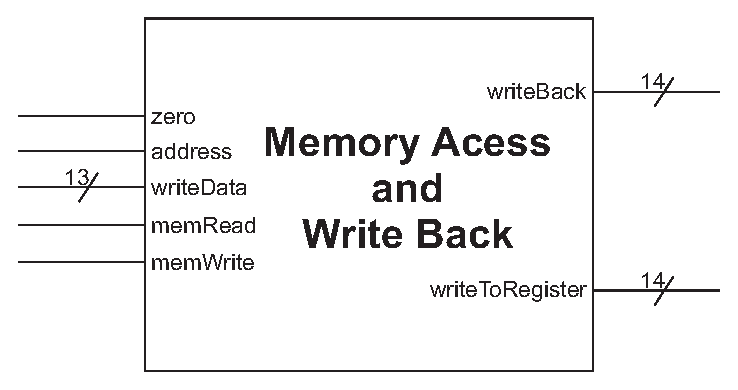
\includegraphics{./datapath/Graphic4.eps}
		\caption*{Datapath dos estágios 4 e 5.}
		\end{center}
	\end{figure}